\documentclass[titlepage]{article}
\usepackage[hidelinks]{hyperref}
\usepackage{indentfirst}
\usepackage{enumitem}
\usepackage{listings}
\usepackage{xcolor}
\usepackage{forest}
\usepackage{tikz}
\usepackage[T1]{fontenc}

\usetikzlibrary{matrix,arrows,shapes}

\lstset{
	basicstyle=
		\def\fvm@Scale{0.8}
		\fontfamily{fvm}\selectfont,
	language=C++,
	tabsize=4
}

\lstdefinestyle{inline-hl}{
	keywordstyle={\bfseries \color{orange}}
}
\lstdefinestyle{display-code}{
	showstringspaces=false,
	commentstyle=\color{gray},
	xleftmargin=2\parindent
}
\lstdefinestyle{more-settings}{
	language=Python,
	numbers=left,
	numberstyle=\ttfamily\color{gray},
	showstringspaces=false,
	morekeywords={True, as},
	xleftmargin=2\parindent,
	keywordstyle={\bfseries \color{orange}}
}



\title{
Homework 1 (Chapter 3) - Due 17th Sep, 2017\\
\begin{large}
Data Structures and Algorithm Analysis in C++
\end{large}
}
\author{Kingsley}
\date{\today}



\forestset{
	forest-style/.style={
		for tree={
			circle, draw,
			every node/.style={
				circle, draw,
				inner sep=0pt,
				text width=6mm,
				align=center
			}
		}
	}
}



\begin{document}
\maketitle

\hypersetup{pageanchor=false}
\clearpage
\tableofcontents
\clearpage
\hypersetup{pageanchor=true}

\section{Basics}
\subsection{Enumerate with alphabet}
\begin{enumerate}[label=(\alph*)]
\item $\Theta(n)$
\item $\Theta(n\log n)$
\item $\Theta(n^2)$
\end{enumerate}

\subsection{Inline code}
\begin{enumerate}
\item \verb|verb| effect: \verb|while (true) i++;|
\item \verb|texttt| effect: \texttt{while (true) i++;}
\item \verb|texttt| with \verb|underline| command: \texttt{\underline{while} (true) i++;}
\item \verb|lstinline| effect: \lstinline{while (true) i++;}
\item \verb|lstinline| with \verb|highlight| option: \lstinline[style=inline-hl]{while (true) i++;}
\end{enumerate}

\subsection{Code block}
\begin{enumerate}
\item Code block effect:
\begin{lstlisting}[style=display-code]
// This is an in-file code block
#include <iostream>

int main()
{
	std::cout << "Hello, World!\n";
	return 0;
}
\end{lstlisting}

\item Code file effect:
\lstinputlisting[style=display-code]{sample.cpp}

\item More settings example:
\begin{lstlisting}[style=more-settings]
try:
	num = int(input(msg))
	passed = True
except ValueError as e:
	print("Please input a number")
\end{lstlisting}
\end{enumerate}

\section{Trees}
\subsection{Binary tree}

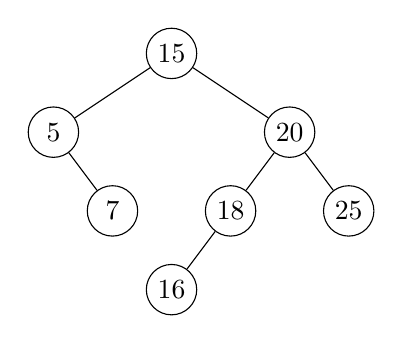
\begin{tikzpicture}[
	every node/.style={
		circle, draw,
		inner sep=0pt,
		text width=6mm,
		align=center
	},
	level distance=10mm,
	level 1/.style={sibling distance=30mm},
	level 2/.style={sibling distance=15mm}
]
\node{$15$}
child { node{$5$}
	child[missing]
	child { node{$7$} }
}
child { node{$20$}
	child { node{$18$}
		child { node{$16$} }
		child[missing]
	}
	child { node{$25$} }
};
\end{tikzpicture}

\subsection{Normal tree}
\subsubsection{With tikz package}
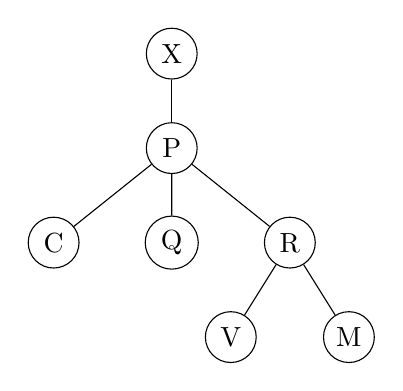
\begin{tikzpicture}[
	every node/.style={
		circle, draw,
		inner sep=0pt,
		text width=6mm,
		align=center
	},
	level distance=1.2cm
]
\node{X}
child { node{P}
	child { node{C} }
	child { node{Q} }
	child { node{R}
		child { node{V} }
		child { node{M} }
	}
};
\end{tikzpicture}

\subsubsection{With forest package}
\begin{forest} forest-style
[, phantom, s sep = 1cm
	[1
		[2[3]]
		[4[5]]
		[6]
	]
]
\end{forest}

\subsection{Forest}

\begin{forest} forest-style
[, phantom, s sep = 1cm
[A
	[B [C] [D[E]] [F]]
	[G]]
[H
	[I]
	[J [K [L]]
	[M [N] [O]]]]
[P
	[Q] [R [S] [T]] [U] [V [W [X]] [Y]] [Z]]
]
\end{forest}

\section{More}
\subsection{Linked list}
\begin{center}
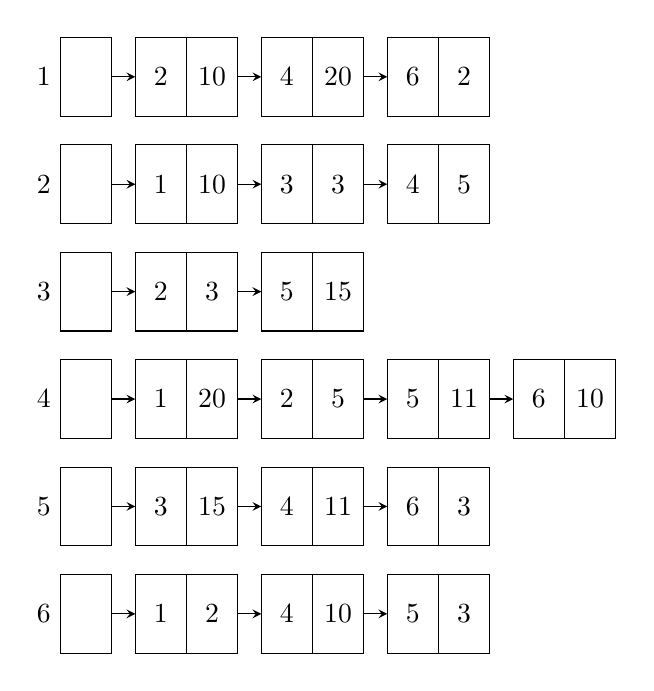
\begin{tikzpicture}[
	circarrow/.style={
		*->, shorten <=-2pt
	}, >=stealth
]
\matrix (M)
[
	matrix of nodes,
	column sep=-\pgflinewidth,
	row sep=3.5mm,
	nodes in empty cells,
	nodes= {
		draw, minimum width=.65cm, outer sep=0pt,
		minimum height=1.0cm, anchor=center
	}
] {
 &[3mm] 2 & 10 &[3mm] 4 & 20 &[3mm] 6 & 2 \\
 & 1 & 10 & 3 & 3 & 4 & 5 \\
 & 2 & 3 & 5 & 15 \\
 & 1 & 20 & 2 & 5 & 5 & 11 &[3mm] 6 & 10 \\
 & 3 & 15 & 4 & 11 & 6 & 3 \\
 & 1 & 2 & 4 & 10 & 5 & 3 \\
};

\foreach \i in {1,2,3,4,5,6} {
	\path (M-\i-1) [late options={label=left:\i}];
	\draw[->] (M-\i-1)--(M-\i-2.west);
	\draw[->] (M-\i-3)--(M-\i-4.west);
}
\draw[->] (M-1-5)--(M-1-6.west);
\draw[->] (M-2-5)--(M-2-6.west);
\draw[->] (M-4-5)--(M-4-6.west);
\draw[->] (M-4-7)--(M-4-8.west);
\draw[->] (M-5-5)--(M-5-6.west);
\draw[->] (M-6-5)--(M-6-6.west);
\end{tikzpicture}
\end{center}

\subsection{Bplus tree}
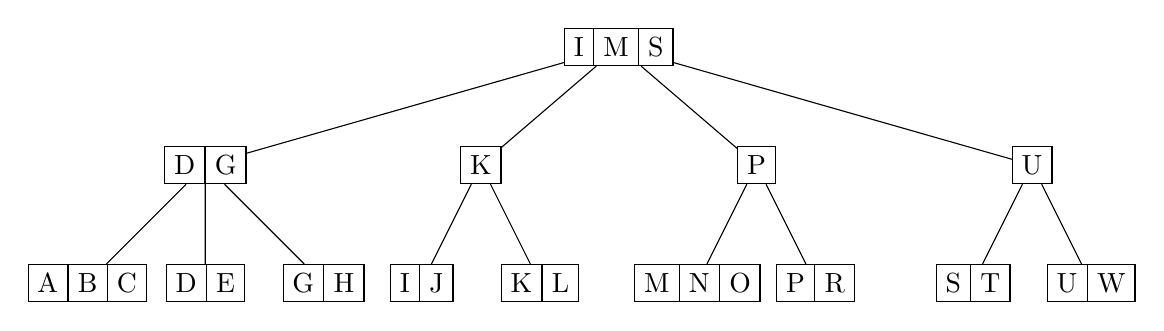
\begin{tikzpicture}
\tikzstyle{bplus-node}=
[
	draw, rectangle split,
	rectangle split horizontal,
	rectangle split ignore empty parts
]
\tikzstyle{every node}=[bplus-node]
\tikzstyle{level 1}=[sibling distance=35mm]
\tikzstyle{level 2}=[sibling distance=15mm]

\node {I \nodepart{two} M \nodepart{three} S} [-]
	child {node {D \nodepart{two} G}
		child {node {A \nodepart{two} B \nodepart{three} C}}
		child {node {D \nodepart{two} E}}
		child {node {G \nodepart{two} H}}
	}
	child {node {K}
		child {node {I \nodepart{two} J}}
		child {node {K \nodepart{two} L}}
	}
	child {node {P}
		child {node {M \nodepart{two} N \nodepart{three} O}}
		child {node {P \nodepart{two} R}}
	}
	child {node {U}
		child {node {S \nodepart{two} T}}
		child {node {U \nodepart{two} W}}
	}
;
\end{tikzpicture}

\end{document}
